
\documentclass[12pt]{article}
\usepackage[utf8]{inputenc}
\usepackage[brazil]{babel}
\usepackage[T1]{fontenc}
\usepackage{lmodern}
\usepackage[a4paper, margin=1in]{geometry}
\usepackage{graphicx}
\usepackage{hyperref}

\title{Normas para infraestrutura de datacenters}
\author{Breno Fernandes - 01169313}
\date{\today}

\begin{document}

\maketitle

\section*{Introdução}
As normas técnicas, como a \textbf{NBR 16665:2019} e a \textbf{ANSI/TIA-942}, são fundamentais para padronizar os critérios de projeto, construção e operação de datacenters, garantindo a integridade dos dados, eficiência e segurança dos serviços de TI. Essas normas estabelecem especificações detalhadas que abrangem desde a infraestrutura física (posicionamento, distância, pisos e sistema de detecção, prevenção e controle de incêndios.) até o impacto ambiental, a eficiência energética e a quantidade de componentes redundantes. Ao definir parâmetros técnicos precisos, as diretrizes asseguram interoperabilidade entre equipamentos, conformidade com requisitos legais e regulatórios, e promovem a adoção de melhores práticas para minimizar riscos operacionais e otimizar o desempenho dos datacenters.

\section*{NBR 16665:2019}
A norma estabelece requisitos para o projeto, construção e operação de datacenters no Brasil, abordando desde infraestrutura física – como layout, pisos elevados e sistemas de combate a incêndios – até critérios ambientais e energéticos. Um diferencial dessa norma é sua ênfase na sustentabilidade, incentivando o uso de energias renováveis e a gestão eficiente de recursos, considerando as características do clima tropical e da matriz energética brasileira. Além disso, detalha parâmetros para controle térmico e umidade, fundamentais para regiões de alta temperatura, e estabelece métricas como o PUE \textit{(Power Usage Effectiveness)} para otimizar o consumo energético. A norma também incorpora exigências legais nacionais, garantindo conformidade com regulamentações trabalhistas e normativas da ABNT.

\section*{ANSI/TIA-942}
Já a ANSI/TIA-942 é um padrão internacional voltado para alta disponibilidade e interoperabilidade global. Sua principal contribuição é a classificação dos datacenters em Tiers (I a IV), definindo níveis de redundância e resiliência. Enquanto um datacenter Tier I possui infraestrutura básica sem redundância, um Tier IV exige tolerância total a falhas, com sistemas 2N+1  — isto é, os componentes críticos são duplicados (2N) com a adição de uma unidade extra (+1) para assegurar a continuidade operacional mesmo durante manutenções ou falhas.  Além disso, a norma especifica diretrizes para cabeamento estruturado, topologias de rede e segurança física, garantindo escalabilidade e integração entre equipamentos de diferentes fabricantes.

\section*{Diferenças e Complementaridades}
A principal diferença entre as normas está no foco geográfico e estratégico. A NBR 16665:2019 atende às especificidades do mercado brasileiro, incorporando desafios climáticos e regulatórios locais. Por outro lado, a ANSI/TIA-942 possui caráter global, sendo adotada por empresas multinacionais que buscam certificações internacionais, como a classificação de Tiers auditada pelo Uptime Institute.

Apesar das diferenças, as normas se complementam ao abordar aspectos distintos: enquanto a ANSI/TIA-942 fornece um framework técnico para garantir disponibilidade e redundância, a NBR 16665:2019 enfatiza sustentabilidade e conformidade legal.

\section*{Diferenças entre Datacenters Tier II e Tier III}
A classificação dos datacenters em Tiers, conforme a ANSI/TIA-942, define níveis crescentes de resiliência e redundância. Entre os níveis, destacam-se as diferenças entre Tier II e Tier III:

\begin{itemize}
    \item \textbf{Datacenter Tier II:} 
    \begin{itemize}
        \item Apresenta redundância parcial dos componentes críticos, proporcionando proteção contra falhas simples.
        \item Possui menos caminhos redundantes, o que pode resultar em interrupções durante manutenções programadas.
        \item Adequado para operações com menor exigência de continuidade ininterrupta.
    \end{itemize}
    \item \textbf{Datacenter Tier III:}
    \begin{itemize}
        \item Possui uma arquitetura de manutenção concorrente, permitindo a substituição ou remoção de componentes sem interromper as operações.
        \item Dispõe de sistemas redundantes e múltiplas rotas de alimentação tanto de rede elétrica quanto de conexão com a rede lógica, assegurando alta disponibilidade mesmo durante manutenções.
        \item Projetado para ambientes de missão crítica -- auqeles que não podem se dar o luxo de parar em nenhum momento.
    \end{itemize}
\end{itemize}

\section*{Considerações Finais}
Embora a decisão quanto à graduação do datacenter deva se fundamentar prioritariamente em requisitos técnicos e operacionais, as implicações financeiras acabam sendo um impeditivo para que a maioria dos datacenters alcancem o nívle de disponibilidade que seria recomendado para a sua operação.
Em síntese, a escolha entre as normas e a graduação dos datacenters deve ser orientada pelas necessidades específicas, pelo escopo do projeto e pelo contexto operacional. Cada norma apresenta características próprias e a decisão quanto à classificação em Tiers envolve tanto considerações técnicas quanto financeiras, de forma a atender de maneira equilibrada os requisitos de desempenho, segurança e eficiência.

\section*{Datacenter Tier III e IV no Brasil}

\subsection*{Surfix Datacenter - Tier III}O Surfix datacenter, localizado aqui em Pernambuco foi o primeiro datacenter do estado a receber a certficação de \textbf{Tier III} pelo \textit{Uptime Institute}.

\begin{center}
  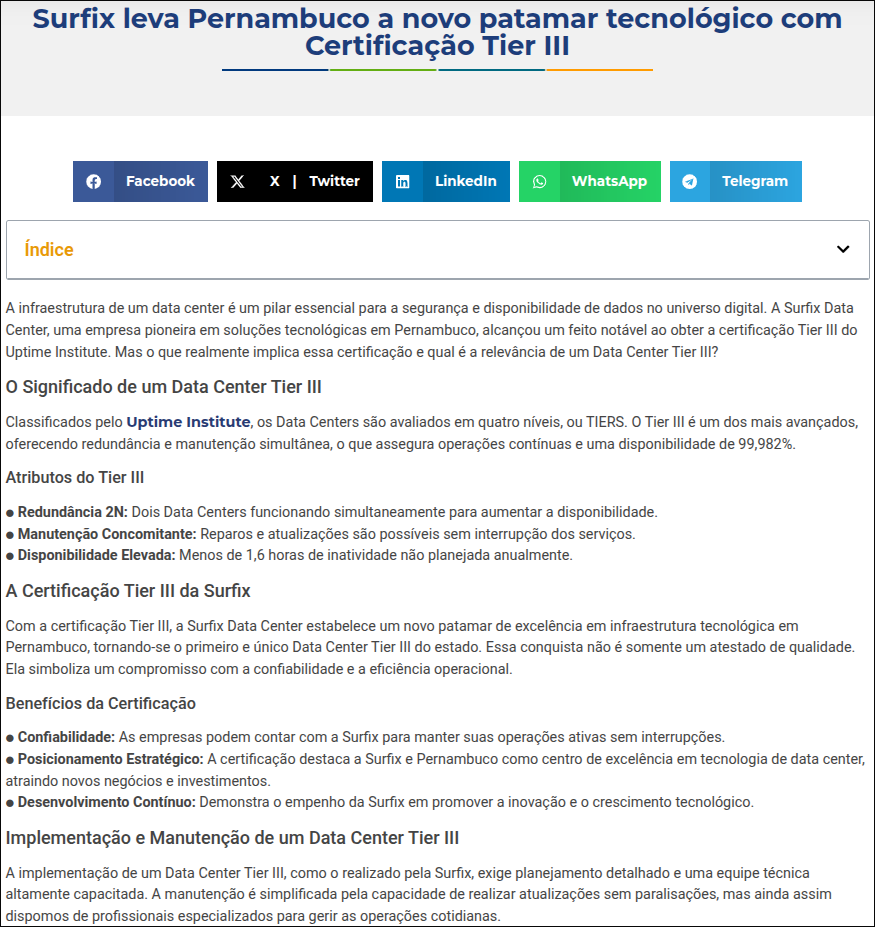
\includegraphics[width=0.8\textwidth]{surfix_noticia.jpg} 
\end{center}

Para mais detalhes, consulte a notícia completa no link: \href{https://surfix.com.br/surfix-data-center-leva-pernambuco-a-um-novo-patamar-tecnologico-com-certificacao-tier-iii/}{Matéria completa}.
\pagebreak{}
\subsection*{Datacenter COP/Telebras - Tier IV}
O Centro de Operações Espaciais Principal (COPE-P), localizado em Brasília foi o segundo datacenter brasileiro a receber a certificação \textbf{Tier IV} do \textit{Uptime Institute}.
\begin{center}
  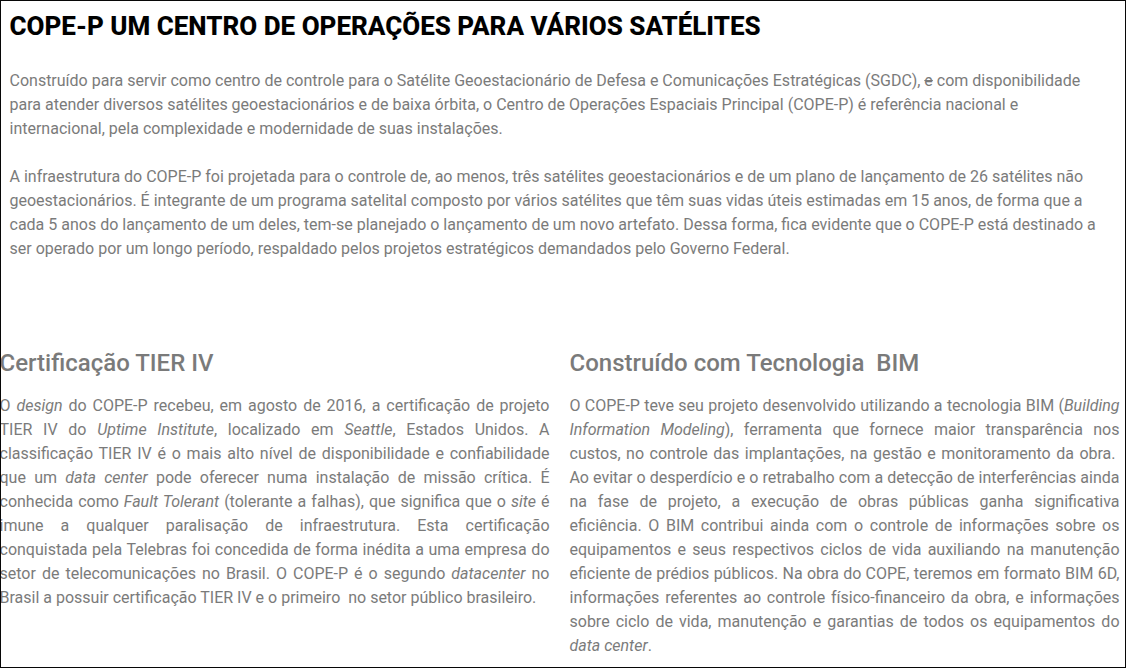
\includegraphics[width=0.8\textwidth]{telebras_noticia.jpg} 
\end{center}

Para mais detalhes, consulte a notícia completa no link: \href{https://www.telebras.com.br/telebras-sat/conheca-o-cope/}{Matéria completa}.

\end{document}
